\documentclass[crop, tikz]{standalone}
\usepackage{tikz}

\usetikzlibrary{positioning, matrix, backgrounds}

\tikzstyle{block} = [rectangle, draw, fill=blue!20, 
    text width=5em, text centered, rounded corners, minimum height=4em]

\definecolor{mygreen}{rgb}{0,0.6,0}
\definecolor{echodrk}{HTML}{0099cc}

\begin{document}
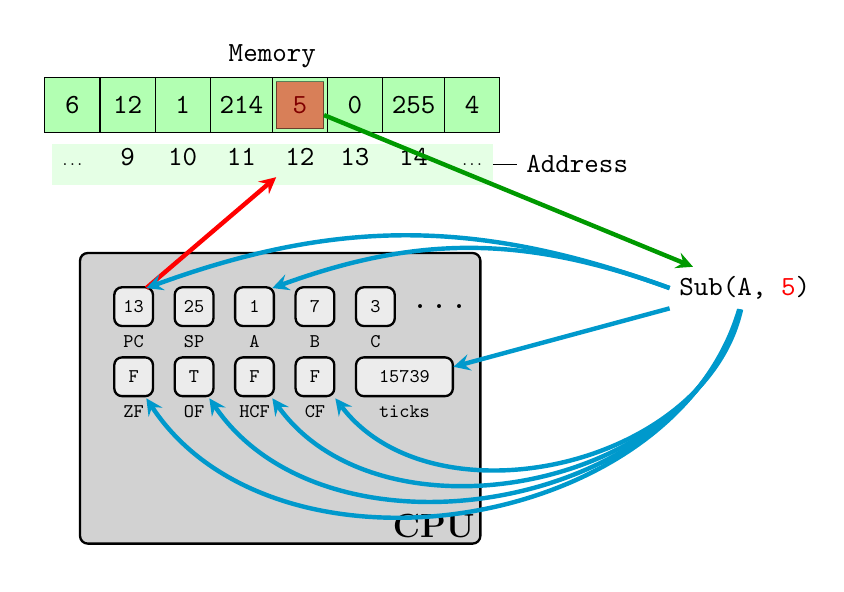
\begin{tikzpicture}[node distance=3cm, auto]
	\draw[opacity=0] (-6, -3.5) rectangle (4, 3.3);
	\begin{scope}[shift={(-4,-2)},transform canvas={scale=0.7}]
		\node [block, color=black, very thick, fill=lightgray!70, minimum height=15em, text width=20em] (cpu) {};
		\node [above left] (lab) at (cpu.south east) {\LARGE \bf CPU};
		\node [below right=2.5em, block, color=black, very thick, fill=lightgray!30, minimum height=2em, inner sep=0em, text width=2em] (PC) at (cpu.north west) {\tt 13};
		\node[below=0.1em of PC] (lPC) {\tt PC};
		\node [right=1em of PC, block, color=black, very thick, fill=lightgray!30, minimum height=2em, inner sep=0em, text width=2em] (SP) {\tt 25};
		\node[below=0.1em of SP] (lSP) {\tt SP};
		\node [right=1em of SP, block, color=black, very thick, fill=lightgray!30, minimum height=2em, inner sep=0em, text width=2em] (A) {\tt 1};
		\node[below=0.1em of A] (lA) {\tt A};
		\node [right=1em of A, block, color=black, very thick, fill=lightgray!30, minimum height=2em, inner sep=0em, text width=2em] (B) {\tt 7};
		\node[below=0.1em of B] (lB) {\tt B};
		\node [right=1em of B, block, color=black, very thick, fill=lightgray!30, minimum height=2em, inner sep=0em, text width=2em] (C) {\tt 3};
		\node[below=0.1em of C] (lC) {\tt C};
		\node [right=0.6em of C] (etc) {\Huge \dots};
		\node [below=1.5em of PC, block, color=black, very thick, fill=lightgray!30, minimum height=2em, inner sep=0em, text width=2em] (ZF) {\tt F};
		\node[below=0.1em of ZF] (lZF) {\tt ZF};
		\node [right=1em of ZF, block, color=black, very thick, fill=lightgray!30, minimum height=2em, inner sep=0em, text width=2em] (OF) {\tt T};
		\node[below=0.1em of OF] (lOF) {\tt OF};
		\node [right=1em of OF, block, color=black, very thick, fill=lightgray!30, minimum height=2em, inner sep=0em, text width=2em] (HCF) {\tt F};
		\node[below=0.1em of HCF] (lHCF) {\tt HCF};
		\node [right=1em of HCF, block, color=black, very thick, fill=lightgray!30, minimum height=2em, inner sep=0em, text width=2em] (CF) {\tt F};
		\node[below=0.1em of CF] (lCF) {\tt CF};
		\node [right=1em of CF, block, color=black, very thick, fill=lightgray!30, minimum height=2em, inner sep=0em, text width=5em] (tkz) {\tt 15739};
		\node[below=0.1em of tkz] (ltkz) {\tt ticks};
			
		\coordinate (PC) at (-0.5, 2);
		\coordinate (A) at (1.1, 2);
		\coordinate (ZF) at (-0.5, 0.6);
		\coordinate (OF) at (0.3, 0.6);
		\coordinate (HCF) at (1.1, 0.6);
		\coordinate (CF) at (1.9, 0.6);
		\coordinate (tkz) at (3.4, 1.0);
	\end{scope}
	\begin{scope}[font=\ttfamily, array/.style={matrix of nodes,nodes={draw, minimum size=7mm, fill=green!30},column sep=-\pgflinewidth, row sep=0.5mm, nodes in empty cells, row 2/.style={nodes={draw=none, fill=none, minimum size=5mm}}}, shift={(-2.9,2)},transform canvas={scale=1.0}]
		\matrix[array,ampersand replacement=\&] (array) {
	6 \&  12 \&  1 \&  214 \&  5 \&  0 \&  255 \& 4  \\
	{\tiny \dots} \& 9 \& 10 \& 11 \& 12 \& 13 \& 14 \& {\tiny \dots}\\};

		\begin{scope}[on background layer]
			\fill[green!10] (array-2-1.north west) rectangle (array-2-8.south east);
		\end{scope}
		\draw[<->, opacity=0.0]([yshift=0mm]array-1-1.north west) -- node[above,color=black, opacity=1.0] {Memory} ([yshift=0mm]array-1-8.north east);

		\node[draw, fill=red, opacity=0.5, minimum size=6mm] at (array-1-5) (box) {};

		\draw (array-2-8.east)--++(0:3mm) node [right]{Address};

		\draw[-stealth, ultra thick, red] (PC) -- (array-2-5);
		\node[] (subi) at (6, -2) {\tt Sub(A, \textcolor{red}{5})};
		\draw[-stealth, ultra thick, mygreen] (box) -- (subi);
		\path[-stealth, ultra thick, echodrk] (subi.west) edge[bend right=20] (A);
		\path[-stealth, ultra thick, echodrk] (subi.west) edge[bend right=20] (PC);
		\draw[-stealth, ultra thick, echodrk] (subi) -- (tkz);
		\path[-stealth, ultra thick, echodrk] (subi) edge[bend left=65] (ZF);
		\path[-stealth, ultra thick, echodrk] (subi) edge[bend left=65] (OF);
		\path[-stealth, ultra thick, echodrk] (subi) edge[bend left=65] (HCF);
		\path[-stealth, ultra thick, echodrk] (subi) edge[bend left=65] (CF);
	\end{scope}
\end{tikzpicture}
\end{document}
